%Tablas hechas con la herramienta http://www.tablesgenerator.com/# cambiando l para p{8cm} para hacer el salto de linea
\documentclass{article}

\usepackage{titlesec}
\usepackage[utf8]{inputenc}
\usepackage{graphicx}
\usepackage{ amssymb }
%\usepackage{subfig}
\usepackage{subcaption}
%\usepackage{breqn}
\usepackage{mathtools,bm}
\usepackage{eurosym}
\usepackage{amstext} % for \text
\DeclareRobustCommand{\officialeuro}{%
  \ifmmode\expandafter\text\fi
  {\fontencoding{U}\fontfamily{eurosym}\selectfont e}}
\usepackage[spanish]{babel} %changes the LaTex default labels to spanish
\usepackage{float} %enables the anchorage of the figures and tables within the text, with [H]
\usepackage{longtable}

\usepackage[a4paper,bindingoffset=0.2in,%
            left=1in,right=1in,top=1in,bottom=1in,%
            footskip=.25in]{geometry}
% \graphicspath{ {images/}, {images2/} }
\usepackage{amsmath}
\usepackage[hyphens]{url}
\usepackage{hyperref}
\usepackage{multirow}


%\setcounter{secnumdepth}{4}

\titleformat{\paragraph}
{\normalfont\normalsize\bfseries}{\theparagraph}{1em}{}
\titlespacing*{\paragraph}
{0pt}{3.25ex plus 1ex minus .2ex}{1.5ex plus .2ex}

\newcommand*{\frontPageEC}[2]{
    \begingroup % Create the command for including the title page in the document
        \centering % Center all text
        \vspace*{\baselineskip} % White space at the top of the page
        {\begin{flushright} \LARGE #1  \end{flushright}}
        \vspace*{\baselineskip}
        \rule{\textwidth}{1.6pt}\vspace*{-\baselineskip}\vspace*{2pt} % Thick horizontal line
        \rule{\textwidth}{0.4pt}\\[\baselineskip] % Thin horizontal line
        {\LARGE #2  \\[0.8\baselineskip] \large{Robótica y Percepción Computacional}}\\[0.2\baselineskip] % Title
        \rule{\textwidth}{0.4pt}\vspace*{-\baselineskip}\vspace{3.2pt} % Thin horizontal line
        \rule{\textwidth}{1.6pt}\\[\baselineskip] % Thick horizontal line
        \vspace*{2\baselineskip} % Whitespace between location/year and editors
        Alumnos: \\[\baselineskip]
        {\Large Luciano García Giordano (150245)} \\
        {\Large Gonzalo Flórez Arias (150048)} \\
        {\Large Salvador González Gerpe (150044)} \\
        
        \vfill
        %\includegraphics[scale=0.4]{UPM.png}
        
        {\itshape Universidad Politécnica de Madrid \\ ETSI Informáticos\par} % Editor affiliation
    \endgroup}

\title{Segmentacion entrega}
\author{Luciano García Giordano, Gonzalo Flórez Arias, Salvador González Gerpe}
\date{24/03/2019}
\date{Universidad Politécnica de Madrid}
\begin{document}

\frontPageEC{24 de marzo de 2019}{Entrega 2 - Segmentación}
\thispagestyle{empty}

\newpage
\tableofcontents
\setcounter{page}{1}

\clearpage
\newpage

\section{Solución propuesta para la segmentación de imágenes}

	A la hora de implementar la parte de segmentación, hemos llegado a tomar una serie de decisiones concretas con el objetivo de lograr los mejores resultados posibles. En este sentido, parecen claras las dos vías por las que se puede optimizar un algoritmo de segmentación: mejorar la calidad de la segmentación y mejorar los tiempos de ejecución.

	Nosotros tuvimos, ya desde el primer momento, claro que lo importante sería lograr una buena calidad en la segmentación, y que a partir de ahí el objetivo sería mejorar los tiempos que tarda el algoritmo en proporcionar la segmentación de cierta imagen (ya que en el robot real esto resulta ser importante). 

	Nuestra primera medida, frente al “diseño” original del algoritmo, fue cambiar el espacio de colores de RGB a HSV. A esto unimos el que finalmente nos quedamos solo con H y S, dejando fuera la V (para tratar de evitar problemas con los cambios de iluminación). Esto resultó ser definitivamente importante para lograr un buen clasificador.

	Para etiquetar las imágenes se usó el programa proporcionado por el profesor, que permite colorear un vídeo abierto con OpenCV, por lo que tomamos algunas imágenes y las coloreamos, tratando de obtener datos variados para la línea, el suelo y las marcas. Con esto construimos nuestro dataset de entrenamiento, con unos 30000 píxeles (lo consideramos una cantidad muy elevada, pero hemos obtenido buenos resultados con ello). Almacenamos, de todas las imágenes coloreadas, los canales H y S de los píxeles coloreados para de ahí entrenar el clasificador.

	Respecto al clasificador, aunque la idea inicial era usar un clasificador euclídeo, de manera similar al desarrollado en la asignatura de Reconocimiento de Formas, pensamos que sería ventajoso buscar algo un poco más complejo pero que pudiera separar mejor las clases. Probamos, usando bibliotecas como sklearn, distintas opciones: primero un clasificador gaussiano de tipo Naïve Bayes, luego una red neuronal de 3 capas, luego una de dos capas (haciendo diversas pruebas con distintos números de nodos en cada capa). Nos quedamos finalmente con una red neuronal de 2 capas con 3 nodos en cada una de ellas. Utilizamos activación logística y una tasa de aprendizaje $\alpha$ de 0.05. Con ello obtenemos unos resultados con altos porcentajes de acierto (99.5\% de acierto usando un 90\% de datos de training y un 10\% de datos de test), pero asegurando a la vez una velocidad de ejecución rápida, que se comentará más adelante.

	Así, al ejecutar el programa se ejecuta el entrenamiento pertinente, y posteriormente se va leyendo el vídeo que se deseé segmentar y calculando dicha segmentación, coloreando y mostrando el resultado a la vez. Es posible también hacer esa lectura directamente a partir de una cámara conectada al ordenador.

	% Pasan a comentarse ahora las mejoras llevadas a cabo desde la primera entrega de segmentación:

	% \begin{itemize}
	% 	\item Gracias a un uso más adecuado de la biblioteca de sklearn, se logró que la ejecución del algoritmo de segmentación fuera paralelizable. De esa manera, no perdemos demasiada potencia de cálculo por utilizar un algoritmo más complejo, como son las redes de neuronas artificiales.
	% 	\item Se pasó a obtener los frames del vídeo de forma reducida. De esa manera, utilizamos para segmentación los píxeles de la imagen de 4 en 4, reduciendo el coste computacional al 1/16 del original. Según nuestras observaciones, casi no se pierde calidad en la segmentación pero se aumenta mucho la velocidad de cómputo.
	% 	\item Se redujeron los nodos en cada capa de la red neuronal, logrando así una velocidad de cómputo mayor sin perder mucha calidad en la segmentación.
	% 	\item Se implementó la parte opcional del seguimiento de la pelota (explicado a continuación).
	% 	\item Como medida para aumentar aún más el acierto en la segmentación, se decidió aumentar la saturación de la cámara a la hora de tomar los vídeos. Según nuestras observaciones, eso hace que los algoritmos funcionen notablemente mejor.
	% 	\item A lo largo de 2 días, tabajamos en el laboratorio de robótica. Allí pudimos grabar y segmentar vídeos tomados desde la propia cámara del robot, con el objetivo de tener ya un vídeo del entorno real de la práctica, además de empezar a probar situaciones reales de seguimiento de líneas en el suelo y de seguimiento de una pelota de ténis.
	% \end{itemize}

	Respecto a la implementación de nuestro programa en Python, al comenzar a ejecutar el programa, se llama al clasificador, y se le pide que entrene a partir de los datos del dataset, que se guardan en un fichero (con datasetGenerator se genera este fichero, a partir de las imágenes coloreadas con etiquetaImagenes. Esa generación solo se hace una vez). 

	Se inicia la captura de imágenes, en base a un vídeo concreto (aunque puede realizarse sobre un vídeo en directo desde una cámara). Cada imagen recibida se reduce en un factor de 4, vertical y horizontalmente (no hemos considerado el trabajar con imágenes algo pequeñas un problema para el futuro, pues el tamaño sigue siendo considerable para poder ver correctamente la línea y cada marca), y en un bucle, se van leyendo las imágenes. Se pasa cada imagen al formato HSV, y se obtiene el H y el S. Se clasifica con predict cada pixel de la imagen con el clasificador, y se muestra por pantalla la imagen segmentada. Entre medias se realizan pruebas del tiempo tardado, usadas para el apartado correspondiente de esta memoria.

\section{Observaciones acerca del límite de upload de Moodle}
	En todos los casos, por el tamaño máximo de la entrega en Moodle, incluimos todos los vídeos convertidos en .m4v (video codec h264) y altamente comprimidos. La calidad es defínitivamente mala, pero al menos podemos incluir varios vídeos de esa manera. A su vez, incluimos el dataset utilizado para entrenar el algoritmo. De esa forma, el evaluador puede ejecutar el programa y observar su comportamiento.

\section{Resultado del algoritmo de segmentación}
	% imagenes representativas y tiempos de ejecucion aqui
	Tras probar el algoritmo que tenemos en el robot de la sala de robótica, podemos certificarnos de que funciona bien en un entorno real controlado. Además, podemos asegurarnos de que los tiempos de ejecución son, como mínimo, adecuados. En nuestro caso, la fase de segmentación se hace de tal forma que conseguimos concluirla en 0.01 segundos, lo que nos permite ejecutar muchos frames en cada segundo (serían 77 si el step que implementamos fuera el total del programa). Si ejecutamos el programa que se entrega en este momento, que no es el brain que desarrollamos para probar en el laboratorio de robótica, el tiempo de ejecución de un ciclo es, de media, de 0,013 segundos en un ordenador portátil similar al del robot del laboratorio de robótica (ambos tienen un procesador Intel i3, por ejemplo). La velocidad de la segmentación fue de 77 frames por segundo.

	En cuanto a resultados, mostramos a continuación algunas capturas que hicimos en el laboratorio de robótica controlando manualmente el robot y capturando el vídeo, y luego procesándolo en nuestro programa. En la figura \ref{fig:figura1} se puede ver que la segmentación es correcta. Sin embargo, los bordes de la línea tienen partes rojas. Eso se debe a que no entrenamos el algoritmo con un dataset demasiado separable. Para solucionar este problema, podemos hacer uso de la función erode de openCV, que nos permite eliminar pequeñas regiones mal clasificadas. Otra solución sería hacer un dataset más variado, aunque dado que no consideramos el contexto del píxel como feature en nuestro algoritmo eso puede no ser suficiente. En un brain que hicimos para probar en la sala de robótica para que el robot pudiera seguir líneas, utilizamos la función erode y obtuvimos resultados excelentes.

	\begin{figure}[H]
	    \centering
	    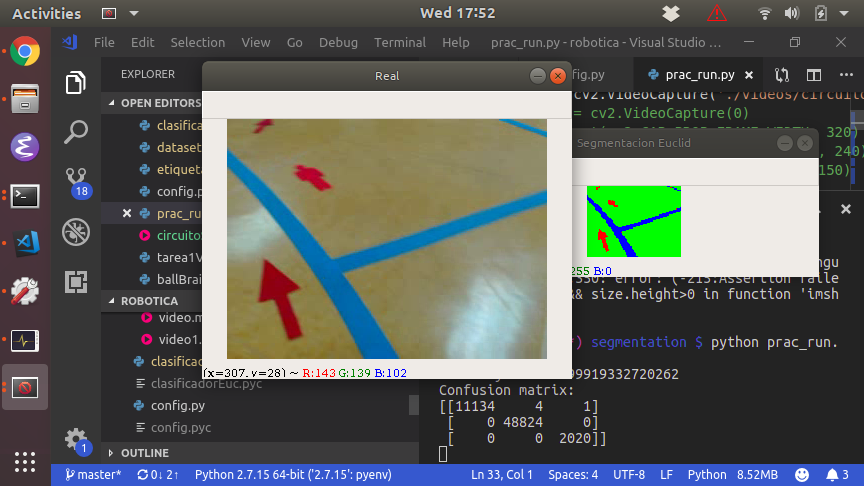
\includegraphics[width=12cm]{./figures/figura1.png}
	    \caption{Ejemplo de la segmentación.} 
	    \label{fig:figura1}
	\end{figure}

	\begin{figure}[H]
	    \centering
	    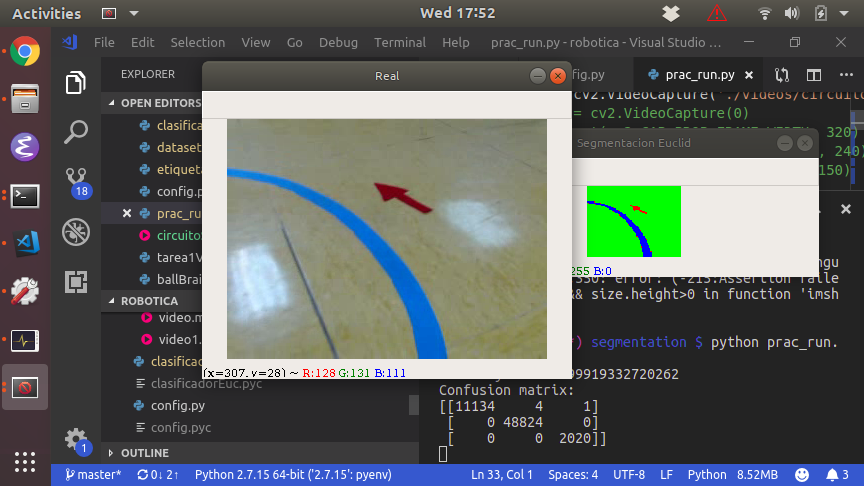
\includegraphics[width=12cm]{./figures/figura2.png}
	    \caption{Ejemplo de la segmentación. Si nos detenemos bien en los bordes de la línea, podemos ver fácilmente algunos píxeles rojos. Sin embargo, hemos llegado a hacer pruebas en el caso de la parte opcional con la función erode de openCV, que nos permite eliminar esas pequeñas regiones mal segmentadas. No implementamos en nuestra solución aún porque eso exige capturar la capa de línea y la de símbolo por separado y en valores binarios para luego aplicar la función a cada una por separado y volver a mostrar los resultados.}
	    \label{fig:figura2}
	\end{figure}

	\begin{figure}[H]
	    \centering
	    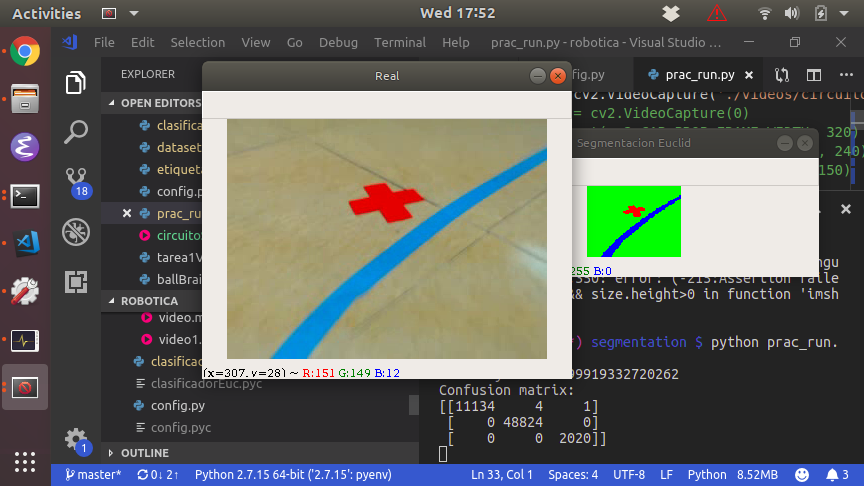
\includegraphics[width=12cm]{./figures/figura3.png}
	    \caption{Ejemplo de la segmentación.}
	    \label{fig:figura3}
	\end{figure}

	\begin{figure}[H]
	    \centering
	    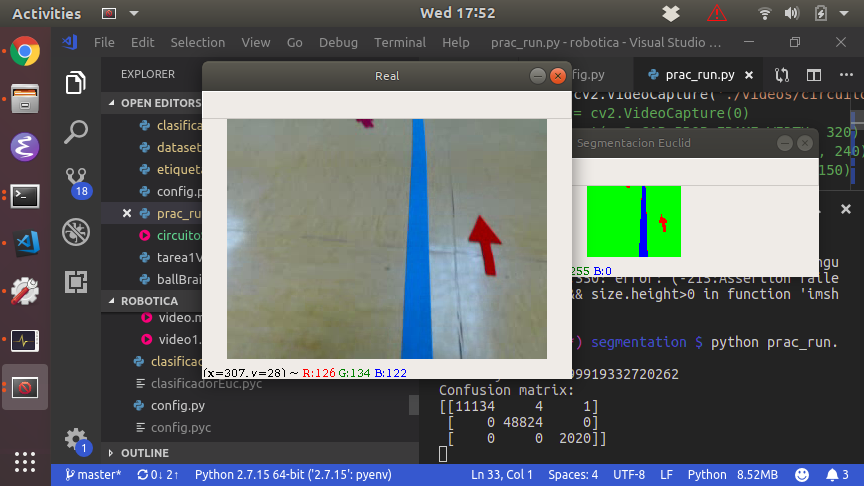
\includegraphics[width=12cm]{./figures/figura4.png}
	    \caption{Ejemplo de la segmentación.}
	    \label{fig:figura4}
	\end{figure}

\section{Descripción del cálculo de la consigna basado en la segmentación de la imagen}
    De manera contraria a lo propuesto en la asignatura, no haremos una clasificación de situaciones entre flechas y líneas para determinar nuestra consigna de control. Lo hacemos porque creemos haber encontrado una solución más general al problema planteado dadas algunas asunciones, listadas a continuación:

    \begin{itemize}
        \item Las líneas que nos proporcionan control (es decir, como mínimo la línea que debemos seguir) son infinitas bajo la percepción del robot en cada momento. De esa manera, una línea siempre genera salida en algún borde de la imagen.
        \item Una de las ``salidas'' generadas por la(s) línea(s) en la imagen es la ``entrada''. La entrada es la línea por la que estamos circulando. Es decir, nuestro ``origen de trayectoria''.
        \item La flecha es suficientemente expresiva como para indicarnos la salida de la imagen dada solamente su dirección. Habiendo contrastado esa asunción en la sala Alpera, podemos afirmar que esta es una asunción razonable respecto a los resultados allí obtenidos.
    \end{itemize}

    Los principales puntos que deben ser observados sobre nuestra solución son los siguientes:
    \begin{itemize}
        \item No haremos una clasificación de situaciones (i.e. cruce en X, curva, recta, ...). Usaremos un método alternativo por nosotros propuesto, que se describirá detalladamente a continuación.
        \item Las flechas serán, para nosotros, equivalentes a cualquier otra figura roja. Y la separaremos de las demás mediante clasificación (se planteará dicha clasificación en la siguiente fase del desarrollo de este proyecto, pero tenemos muy claro que un clasificador, por complejo que tenga que ser, es capaz de separar flechas de las demás clases de forma fiable - en último caso, no descartamos el uso de Deep Learning y un extensivo dataset como suele ser necesario en este tipo de casos para ello)
    \end{itemize}

    Proponemos, por tanto, un método para el cálculo de la consigna desacoplado de situaciones ``estándar''. Según nuestras observaciones, nuestro método es suficientemente general, bajo nuestras asunciones, para permitir no necesitar saber si se trata de un cruce o una curva para navegar el robot adecuadamente por la sala.

    Nuestro método está compuesto por una serie de pasos. Comenzamos con una imagen segmentada en la que conocemos todos los puntos ocupados por líneas y, posiblemente, una figura (asumiremos en esta entrega que es una flecha).

    \subsection{Detección de salidas de la línea de la imagen}
        El primer paso es detectar las intersecciones entre las líneas y el borde de la imagen. Con eso, obtenemos un listado de salidas de la imagen. En nuestra implementación, solo nos quedamos con los puntos centrales de cada intersección (sus coordenadas). Además, en las esquinas, analizamos la intersección de líneas de cada borde adyacente para determinar si se trata de una misma línea o dos separadas. Con eso, no tenemos problemas con salidas que se expresan en más de un borde de la imagen. Como se puede ver en la Figura \ref{fig:consigna2}, obtenemos, a partir de una situación hipotética mostrada en la Figura \ref{fig:consigna1}, las salidas de la imagen.

        \begin{figure}[]
            \centering
            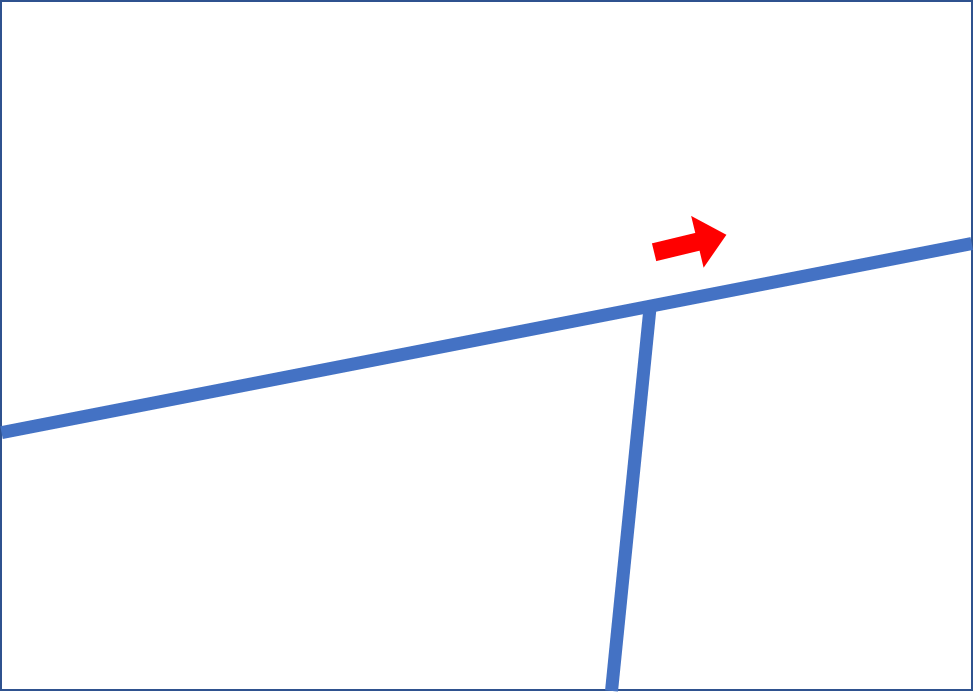
\includegraphics[width=9cm]{figures/consigna1.png}
            \caption{Situación hipotética de cruce en T y flecha}
            \label{fig:consigna1}
        \end{figure}

        \begin{figure}[]
            \centering
            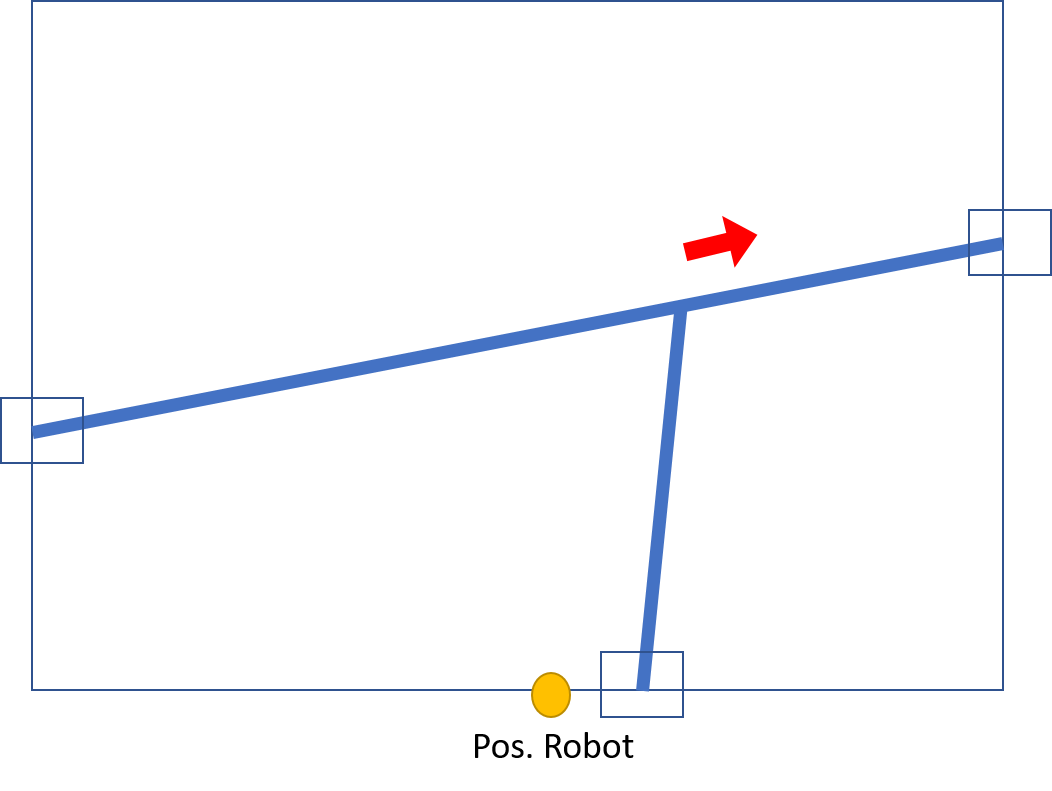
\includegraphics[width=9cm]{figures/consigna2.png}
            \caption{Detección de salidas en una situación hipotética de cruce en T y flecha. Los rectángulos dibujados alrededor de la salida sirven para evidenciar la detección y solo están presentes en esta explicación de nuestro modelo}
            \label{fig:consigna2}
        \end{figure}

    \subsection{Elección de la entrada entre las salidas}
        El siguiente paso para la definición de la consigna de control del robot es la determinación de la entrada a partir de las salidas.

        Dada la lista de coordenadas que corresponden a salidas en nuestro modelo, tenemos que encontrar aquella más cercana al origen del movimiento del robot. Esa será la entrada (punto de referencia de la línea por la que circulamos). En nuestro caso, definimos el origen de movimiento como el punto central inferior de la imagen.

        En la Figura \ref{fig:consigna3}, podemos observar que la salida inferior es la más cercana al origen de movimiento del robot. Por tanto, es la entrada.

        \begin{figure}[H]
            \centering
            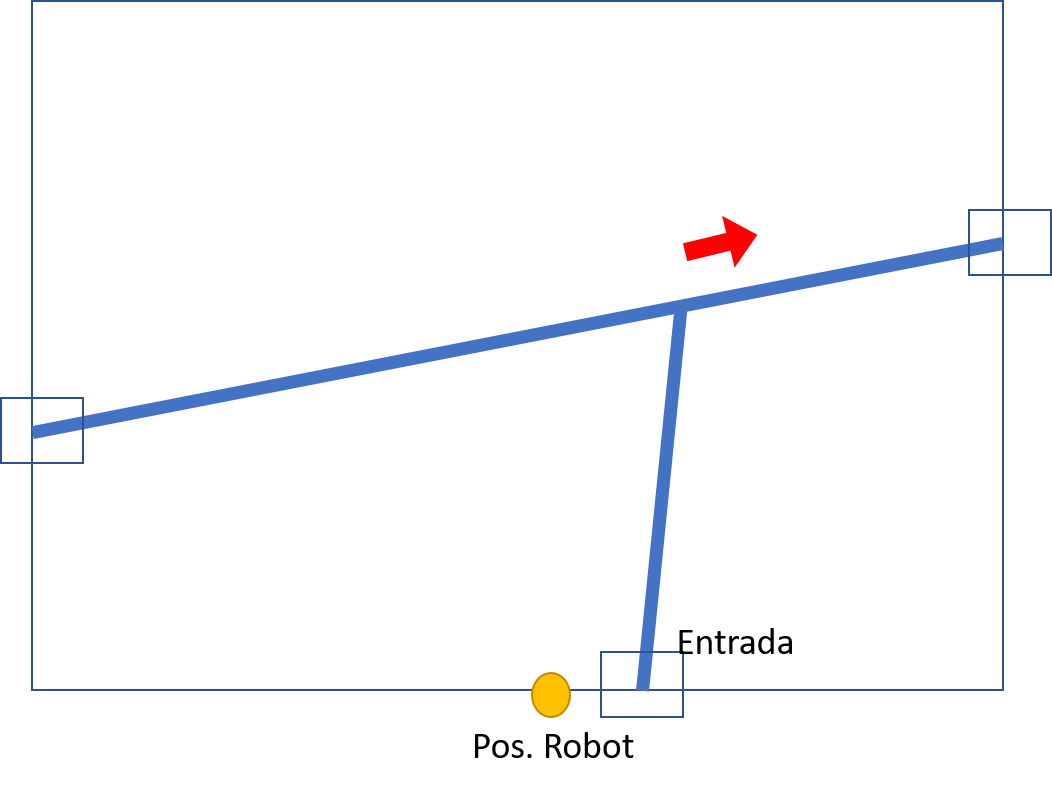
\includegraphics[width=9cm]{figures/consigna3.png}
            \caption{Detección de la entrada, que es una de las salidas en una situación hipotética de cruce en T y flecha. Los rectángulos dibujados alrededor de la salida sirven para evidenciar la detección y solo están presentes en esta explicación de nuestro modelo}
            \label{fig:consigna3}
        \end{figure}


    \subsection{Elección de la salida a tomar}
        \subsubsection{En existencia de sólo una salida}
            En el caso de una salida, no hay que decidir. Simplemente, se salta al siguiente paso con la única salida existente.

        \subsubsection{En existencia de flecha} 
            Para elegir la salida a tomar en caso de tener una flecha representada en la imagen segmentada, calculamos los ángulos entre el vector que define la flecha y los vectores que van desde el centro de la flecha hasta cada una de las salidas. El menor de estos ángulos corresponde a la salida a tomar. En la práctica hemos comprobado que este método es bastante eficaz, y en la mayoría de casos estima correctamente cuál de las dos salidas es por la que debe ir el robot siguiendo correctamente la flecha. En la Figura \ref{fig:consigna5}, podemos observar esa elección.

            \begin{figure}[H]
                \centering
                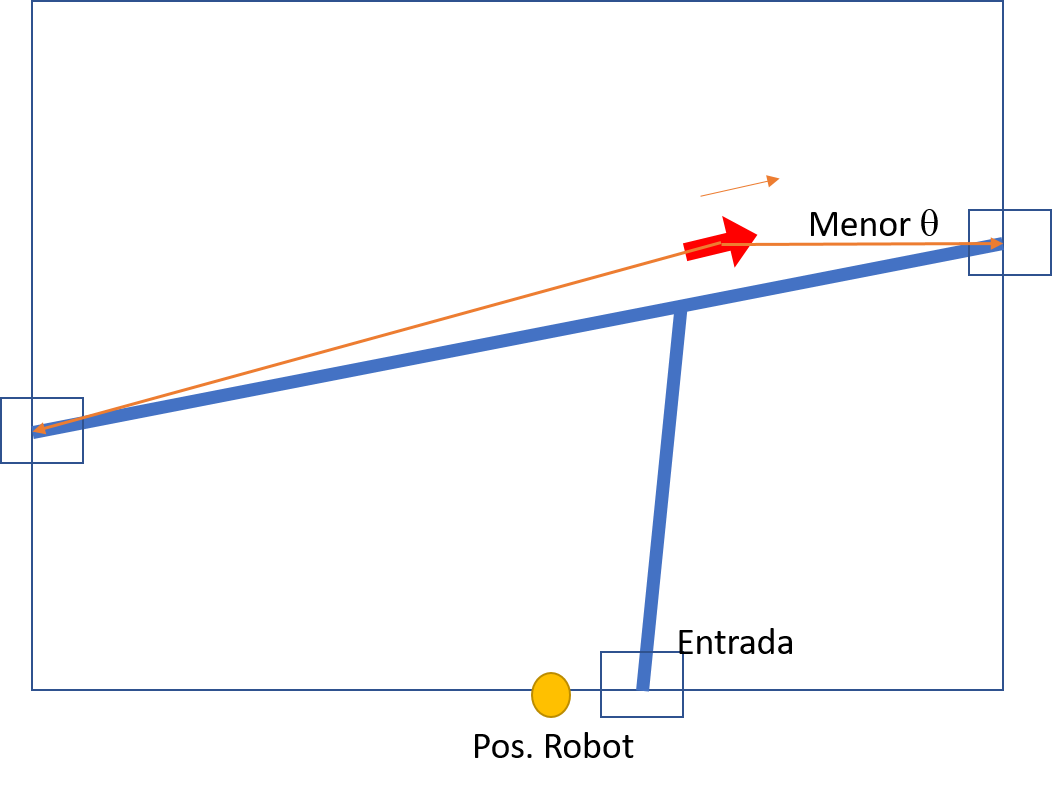
\includegraphics[width=9cm]{figures/consigna5.png}
                \caption{Decisión de la salida a tomar, dada una situación en que hay más de una salida y una flecha.}
                \label{fig:consigna5}
            \end{figure}
        
        \subsubsection{En ausencia de flecha}
            En el caso de tener más de una salida y no disponer de una flecha, la solución más razonable es seguir por la opción más central. Por tanto, elegimos la salida a tomar con base en la distancia al centro superior de la imagen segmentada.

    \subsection{Cálculo de la consigna}
        Para calcular la consigna, definimos en primer lugar un vector entre nuestra entrada y la salida elegida. En la Figura \ref{fig:consigna6}, se ilustra dicho vector.

        \begin{figure}[H]
            \centering
            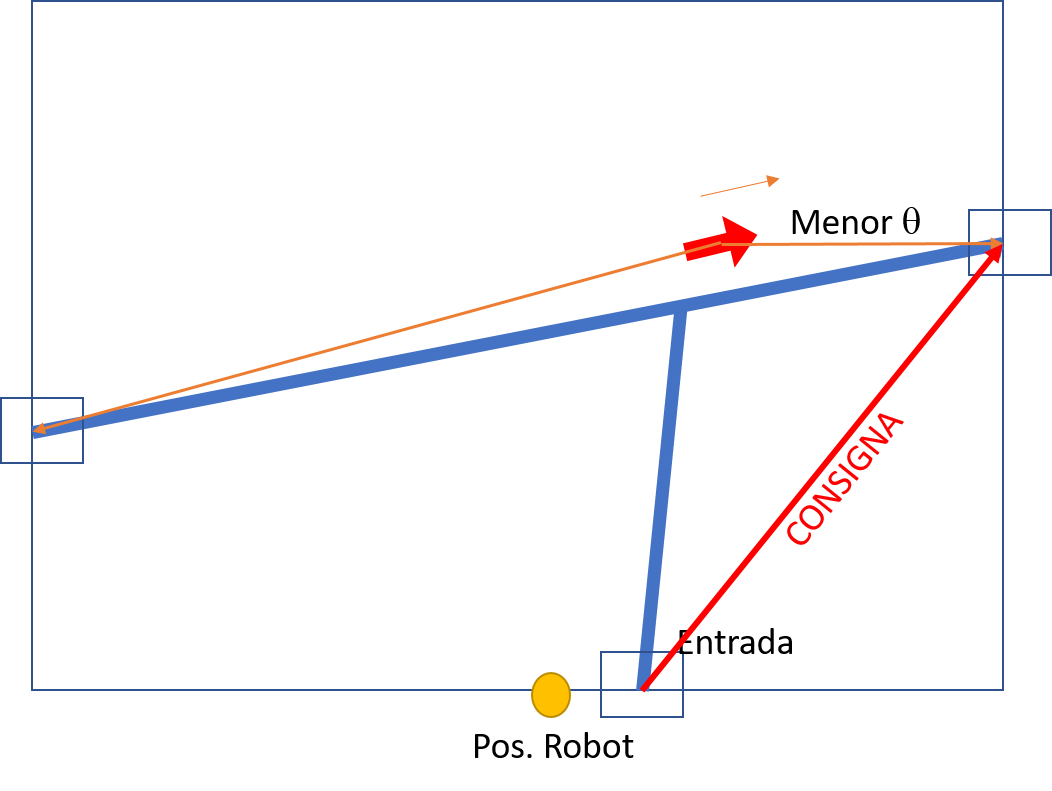
\includegraphics[width=9cm]{figures/consigna6.png}
            \caption{Como se puede observar, utilizamos un vector como orientativo para el cálculo de la consigna.}
            \label{fig:consigna6}
        \end{figure}

        Para calcular la consigna en si, utilizamos la distancia entre los orígenes del robot y del vector y el ángulo entre el vector y la vertical, como se puede ver en la Figura \ref{fig:consigna7}.

        \begin{figure}[H]
            \centering
            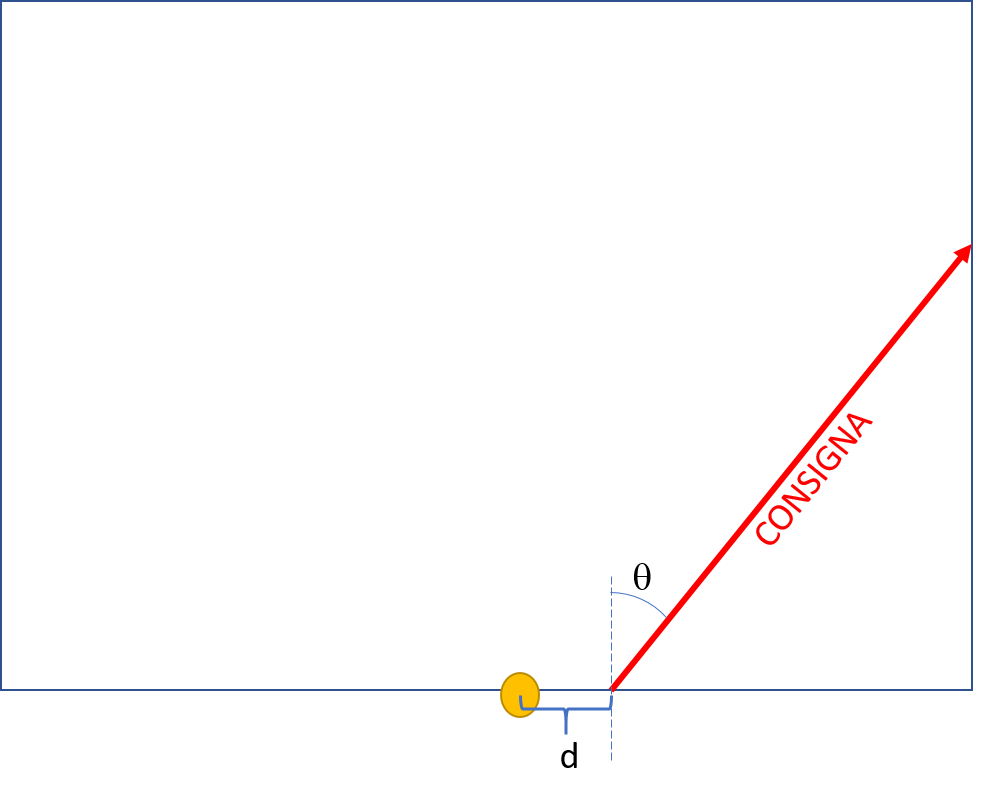
\includegraphics[width=9cm]{figures/consigna7.png}
            \caption{Las medidas $d$ y $\theta$.}
            \label{fig:consigna7}
        \end{figure}
        
        La consigna de giro se calcula mediante la siguiente fórmula:

        $$\delta = \text{giroAnterior} - \theta \times 0.7 + d \times 0.3$$

        $$giro = \frac{\theta \times 0.03 + d \times 0.01}{|\delta \times 0.2|}$$

        La consigna de avance se calcula mediante la siguiente fórmula:

        $$avance = -0.5 \times |giro| + 1$$

        Para el cálculo del giro utilizamos la consigna con valor real y derivada. Para la de avance aprovechamos el efecto de la derivada en el giro también para el avance. Los valores fijos, como $0.2$ en $giro$ y $0.5$ en avance son parámetros. De hecho, el primer de ellos es el $Kd$ de la consigna de giro. En todo caso, esos parámetros todavía no están perfectamente optimizados para el robot en la sala. Sin embargo, presentan valores plausibles para el cálculo de las consignas de control.

\section{Parte opcional. Seguimiento de pelota}
	También realizamos la parte opcional de la práctica, referida al seguimiento de un objeto esférico por parte del robot, que va controlando su distancia a dicho objeto según los resultados del tamaño de la pelota relativo a la cámara del robot. Logramos adaptar el algoritmo de segmentación para poder obtener la pelota de un vídeo, y calculamos la manera de obtener la distancia relativa de la cámara a la pelota, en base a la explicación dada en clase. También hemos realizado una primera integración de esto con la parte de control, de tal manera que el robot se acerque a la pelota si la encuentra a lo lejos y se aleje si la tiene muy cerca. También implementamos la capacidad del robot de girar para intentar mantener la pelota en el centro de su campo de visión. Probamos el algoritmo en forma de “Brain” en el robot del laboratorio de robótica, logrando unos resultados interesantes. Incluimos en la carpeta de entrega un video de demostración del seguimiento junto con la segmentación hecha por el mismo programa.

	Sobre nuestras pruebas en el laboratorio, incluimos en la carpeta de entrega un timelapse grabado con el móvil de uno de los integrantes del grupo guiando el robot por la sala. Además, incluimos dos videos, uno con la imagen original y otro de la segmentación, hechos en directo por el robot en una situación similar a la mostrada en el time lapse (hemos perdido la referencia de si se trata de la misma ejecución o no). Se muestra a continuación una captura de pantalla del video mencionado, tanto de la imagen original (Figura \ref{fig:pelota1}) como de la segmentación (Figura \ref{fig:pelota2}).

	\begin{figure}[H]
	    \centering
	    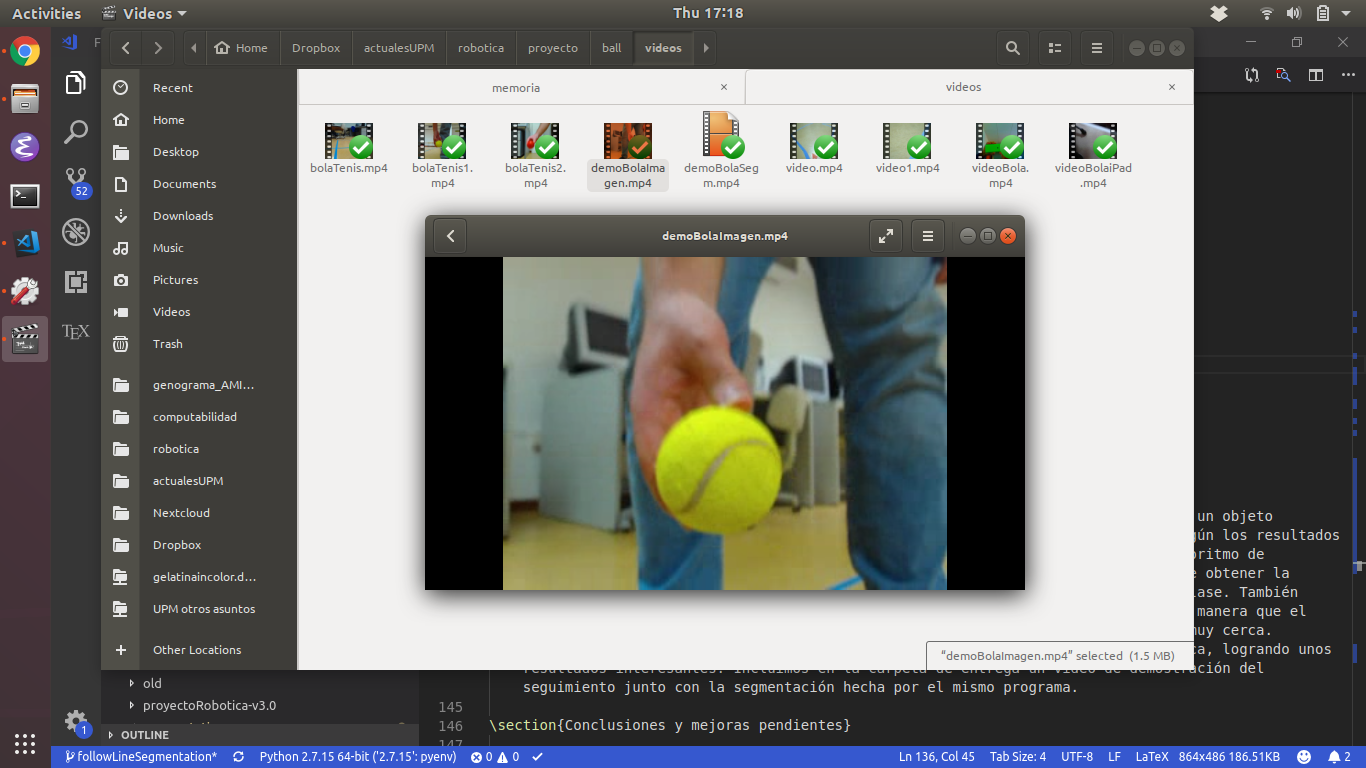
\includegraphics[width=12cm]{./figures/pelota2.png}
	    \caption{Captura de la imagen original de la pelota en un brain que ejecuta en el robot real.}
	    \label{fig:pelota1}
	\end{figure}

	\begin{figure}[H]
	    \centering
	    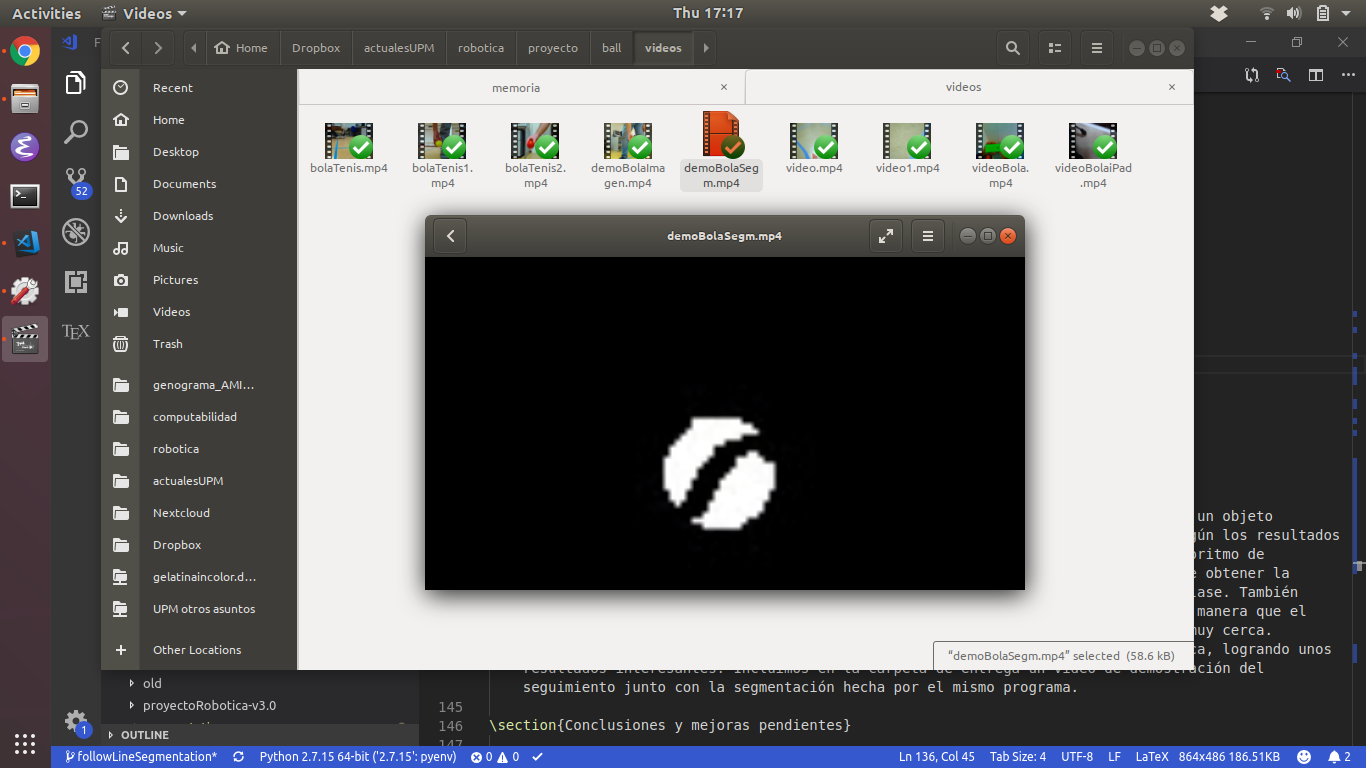
\includegraphics[width=12cm]{./figures/pelota1.png}
	    \caption{Captura de la segmentación de la pelota en un brain que ejecuta en el robot real. Como bien se puede ver, la curva blanca de la pelota de tennis no se captura como parte de la pelota. Además, esa línea crece en la segmentación. Eso es un efecto de la función erode de OpenCV, que usamos príncipalmente para que no se consideren pequeños defectos de la segmentación.}
	    \label{fig:pelota2}
	\end{figure}

\section{Conclusiones y mejoras pendientes}

	Pensamos, en conclusión, que nuestro algoritmo de segmentación obtiene buenos resultados con las pruebas llevadas a cabo. Es cierto que podría ser más rápido (especialmente en nuestra primera versión, de la primera entrega de esta parte), pero hemos tratado de encontrar un equilibrio entre resultados y tiempos de ejecución que nos permita emplear este algoritmo una vez usemos el robot real.
	
	En cuanto a mejoras pendientes, pensamos que diversos puntos requieren nuestra atención. El principal de ellos es que la segmentación todavía está lejos de ser perfecta. Eso se debe principalmente a que un píxel, en su individualidad, no es capaz de expresar del todo bien la entidad a que pertenece. Pensamos utilizar esos datos de segmentación para entrenar un clasificador basado en contexto, que como mínimo pueda fijarse en los píxeles alrededor del que intenta clasificar. Una posibilidad un poco lejana, dada la potencia de cálculo que tiene el robot, sería utilizar un segmentador mediante una red de neuronas artificiales con capas convolucionales. Según nuestro análisis, sería necesaria una capa convolucional al principio y probablemente algunas de pooling o convolución más. Estimamos un total de 3 o 4 capas, lo que ya sería demasiado para el robot que disponemos, además que exigiría operar con bibliotecas bastante complejas (aunque tenemos algo de conocimiento de algunas, como Tensorflow con Keras). Además, eso nos requeriría hacer un dataset mucho más extenso. Intentaremos, sin embargo, hacer esta mejora en el futuro.








% \begin{figure}[H]
%     \centering
%     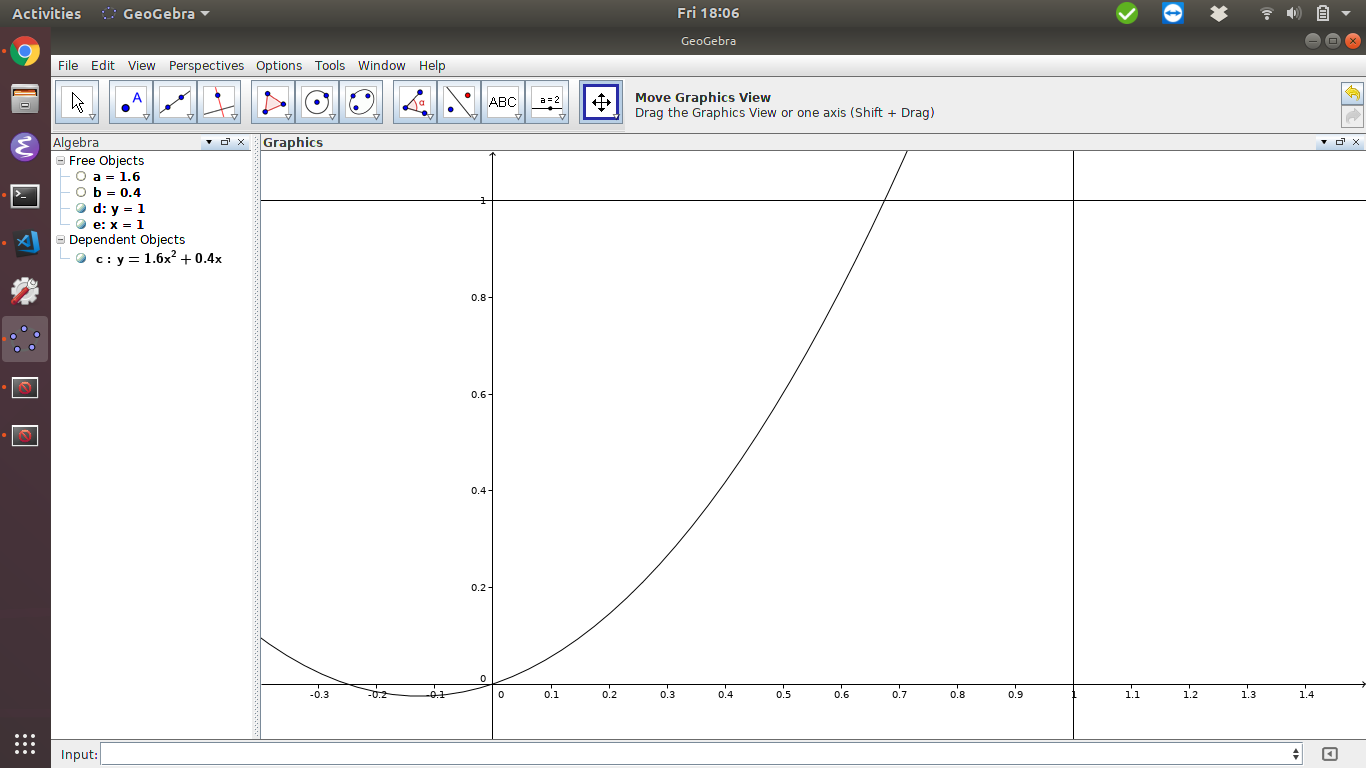
\includegraphics[width=12cm]{modeloCuadratico.png}
%     \caption{Observamos el modelo cuadrático en el software GeoGebra para determinar los parámetros iniciales para nuestra exploración. Con el simulador, los hemos cambiado según nuestras observaciones para que fuera más adecuado al funcionamiento del robot.}
%     \label{fig:modeloCuadratico}
% \end{figure}

\end{document}
